% This file is iccc.tex.  It contains the formatting instructions for and acts as a template for submissions to ICCC.  It borrows liberally from the AAAI and IJCAI formats and instructions.  It uses the files iccc.sty, iccc.bst and iccc.bib, the first two of which also borrow liberally from the same sources.


\documentclass[letterpaper]{article}
\usepackage{iccc}

\usepackage{graphicx}
\usepackage{times}
\usepackage{helvet}
\usepackage{courier}
\pdfinfo{
	/Title (Anything2vec: generalizing word2vec via the use of meaningful contexts)
	/Subject (Proceedings of ICCC)
	/Author (ICCC)}
% The file iccc.sty is the style file for ICCC proceedings.
%

\title{Anything2vec: generalizing word2vec via the use of meaningful
	contexts}
% Add something about its application to trope description - JJ 
%\author{Dan Ventura\\
%Computer Science Department\\
%Brigham Young University\\
%Provo, UT 84602  USA\\
%ventura@cs.byu.edu\\
%}
\setcounter{secnumdepth}{0}

\begin{document} 
	\maketitle
	\begin{abstract}
		\begin{quote}
			% From the old paper:
			%   Word2vec has been a very successful algorithm that is able to give a
			% semantic representation to words on a corpus based in the context
			% they appear. In this paper we will try to extend this concept to
			% other {\em unordered} contexts. We will try to define this context
			% for movie (and TV) tropes.
			In this paper we present a generalized approach to extend the use of word2vec for non traditional NLP (Natural Language Processing). In order to exemplify the idea we use tvtropes dataset (trope names and film names only) to create a text corupus in order to give contextual information to any pice of data.
		\end{quote}
	\end{abstract}
	
	% From the old paper:
	% What are tropes and why we are interested
	
	% We need to find an embedding for tropes that allows us to do trope arithmetic and also process them, and movies in which they are used, in an uniform way.
	
	% We propose trope2vec
	
	% We analyze how it allows to explore the trope space and find
	% similarities between them.
	
	\section{Introduction}
	
	% Motivation: we need to have a representation that is
	% * That includes the context of the trope
	% * relatively compact
	% * capable of doing arithmetic
	% * uniform for tropes and movies.
	
	This work aims to find a knowledge representation and a new methodology to apply machine learning techniques to tropes and films from tvtropes.org in order to discover hidden conections between Tv Tropres entities. That representation and methodology will let us, for example, to discover wich set of tropes will be affordable to create a new block buster film or a new best seller book.   
	
	Tv Tropes (tvtropes.org) is a collaborative website created in 2004 to share information about tips, narrative or cinematographic techniques used in creative works such as movies, tv series, advertaising, videogames, sports, comics or books. Tvtropes.org defines "tropes" as: "A trope is a storytelling device or convention, a shortcut for describing situations the storyteller can reasonably assume the audience will recognize." Articles to describe tropes are writed usually with a very expresive and non formal vocabulary. Each film, tv serie or other fiction element usually include a description and a list of asociated tropes. Tropes pages usually contains a description followed by a list of films or a narrative resource that uses this trope.
	
	To represent tropes we decided to use embeedings vectors for each trope. This representation should allow us to perform concept arithmetic. This property will be very interesting since our goal is to determine, for example, which group of tropes must have a successful film. Applying arithmetic of concepts about tropes we could, for example, find classic western movies, which have their main narrative characteristics, but the western one is replaced by space adventure trope. in order to obtain the set of embeeding vects associated with the tropes we will use word2vec \cite{mikolov2013}. Since the development of this technique in 2013 word2vec is one of the techniques for the generation of embeeding vectors from natural language (NLP) most used. However word2vec has not only been used to obtain embeeding vectors of texts in natural language. Other works like \cite{kazama2018} have shown that it is possible to use word2vec to obtain vectors from non-NLP information sources. Our approach is based on the use of the fundamental elements of information (in our case the tropes) to generate an artificial narrative or corpus that can give a similar meaning to the concepts that they would have in a text written by humans. This artificially created text should represent the relationships between entities in the same way that a human would relate them in a descriptive text about these entities. If the artificial corpus is correctly constructed, it should produce some embeeding vectors with the capacity to offer us a correct arithmetic of concepts. \\
	To achieve this artificial corpus, what we will do will be to place close to those concepts that are related in some way to the specific problem being treated. In the example of tvtropes, we will generate the artificial corpus generating phrases that place the related tropes close. For our specific problem, the tropes that should appear closer will be those that appear in the same movie. So for our example the relationship that will serve as a link between the elements is the relationship of the trope's appearance in the same movie. In order to generate the corpus we will select films that have a maximum of 15 tropes. We take this initial limit since we will generate all the variations without repetitions of 15 elements taken in groups of n elements. his method can give us a corpus of sufficient size to train the model using the word2vec algorithm. \\
	In order to generate the artificial corpus we have followed this procedure. Firstly, we have downloaded all the tvtropes information related to movies and their associated tropes. Next we have selected those films that have a maximum of 15 tropes and eliminating those that have zero tropes. This filtering process generates a reduced set of tropes. The subset of tropes that appear in films with 15 tropes or less, have 6524 unique tropes, full set of tropes have 25405. Figure  \ref{fig:tropesdistributionasociatedtofilms} shows the accumulative distribution of tropes and films, where 250 thresold will include more than 25000 tropes. In our case choosing films with 15 tropes or less the subset have only 6524 but including 99,2 percent of the 250 most popular tropes, so we can consider it a representative subset.\\
	
	\begin{figure}
		\centering
		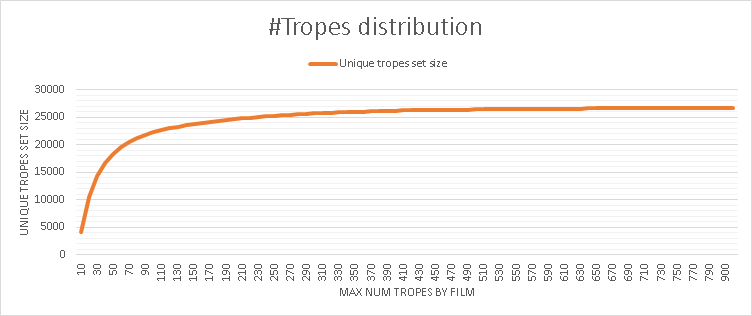
\includegraphics[width=0.9\linewidth]{../images/tropes_distribution_chart.png}
		\caption{Accumulative distribution of tropes dassociated to films}
		\label{fig:tropesdistributionasociatedtofilms}
	\end{figure}
	
	After apply word2vect to a text corpus, a set of embeedings vectors will be created. The embeeding vector have information about the context of a certain word and it is easy to find the relationships with other terms in corpus. The challenge now is how to create a corpus that will be usefull to find relationships between tropes and films. Each film have a description and a list of tropes, and each trope have a description and a list of films that uses this trope. Initially our dataset obtained from tvtropes.org 13th december 2019 included 12360 films and 26742 different tropes (25405 after remove duplicates). The film with higher number of tropes has 1028 tropes and the film with minimum number of tropes has 0 tropes. 673258 pairs film-trope. 73917 duplicate values in pairs. 
	
	
	\begin{center}
		\begin{figure}
			\centering
			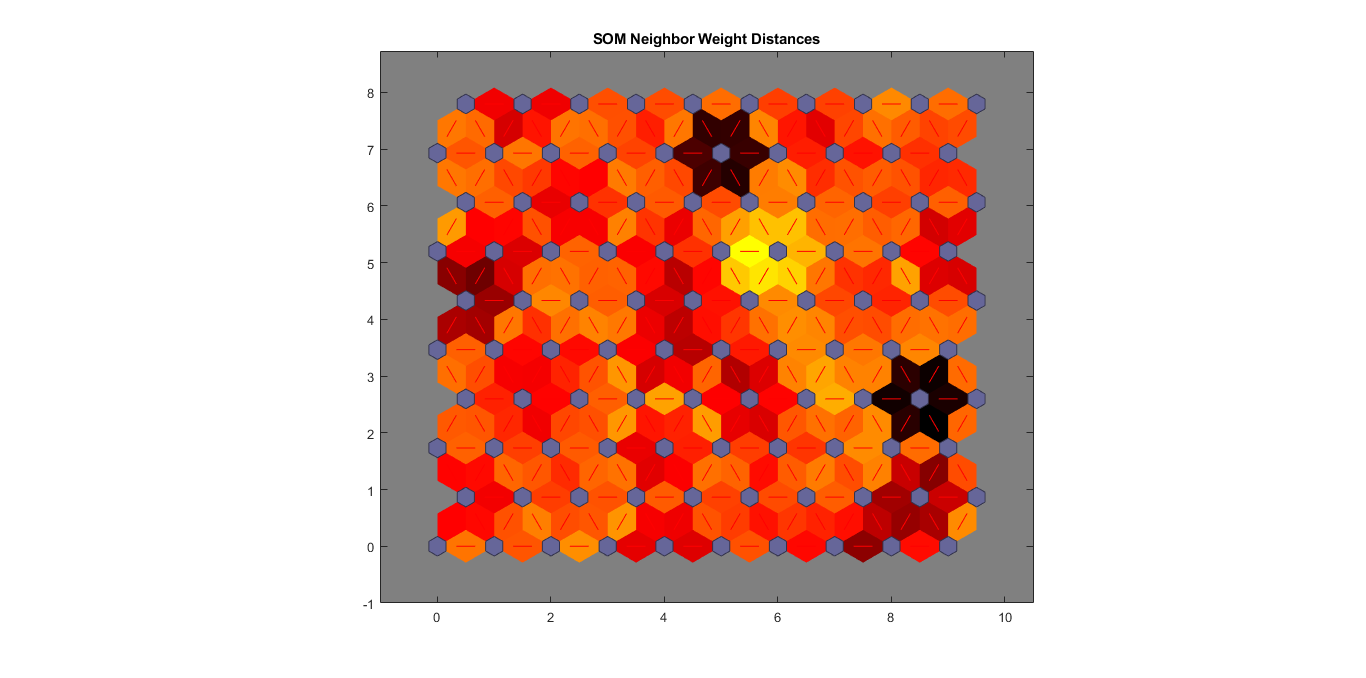
\includegraphics[width=1.25\linewidth]{../images/som_matlab_tropes_15_9}
			\caption{SOM from tropes vectors generated by word2vec}
			\label{fig:sommatlabtropes159}
		\end{figure}
	\end{center}
	
	
	\begin{figure}
		\centering
		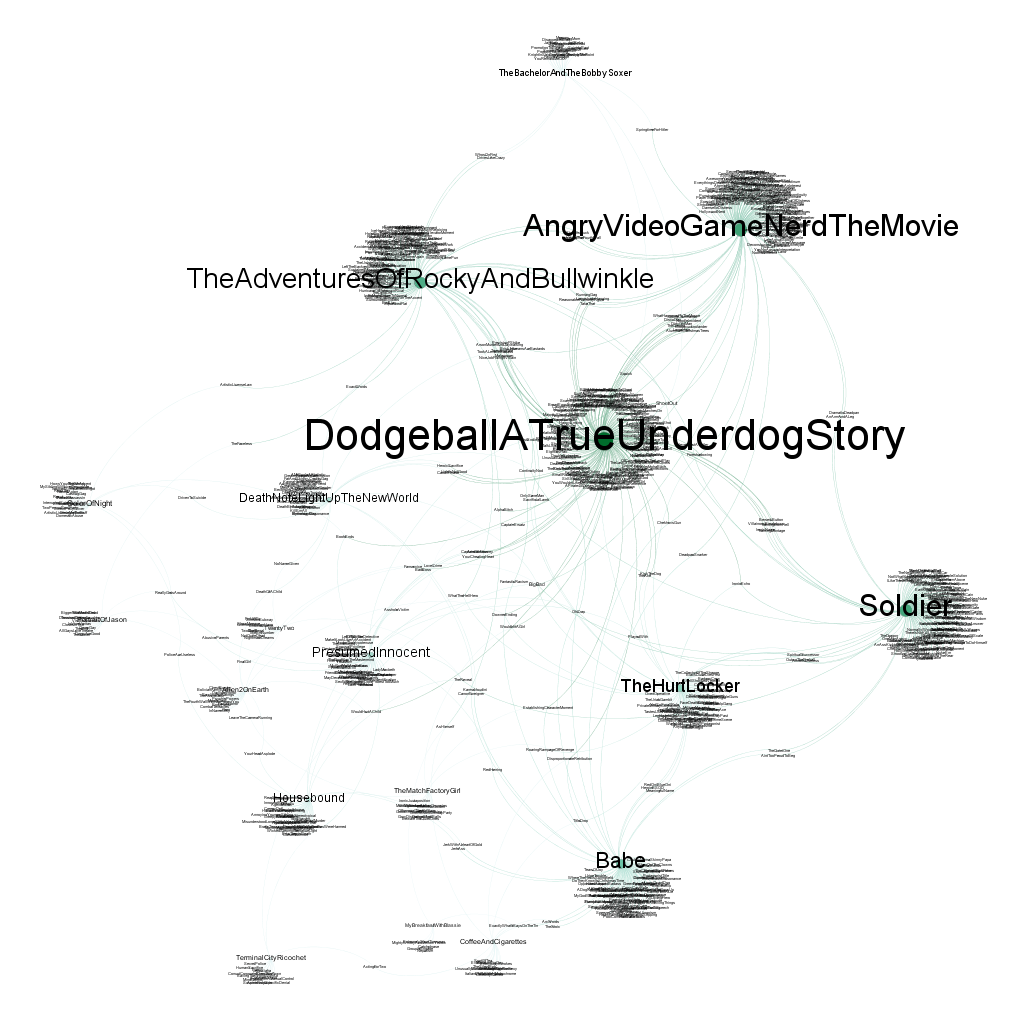
\includegraphics[width=0.9\linewidth]{../data/gephi/pairs_films-trope_1k_v3}
		\caption{}
		\label{fig:pairsfilms-trope1kv3}
	\end{figure}
	
	
	
	
	
	% \begin{figure}
	% 	\centering
	% 	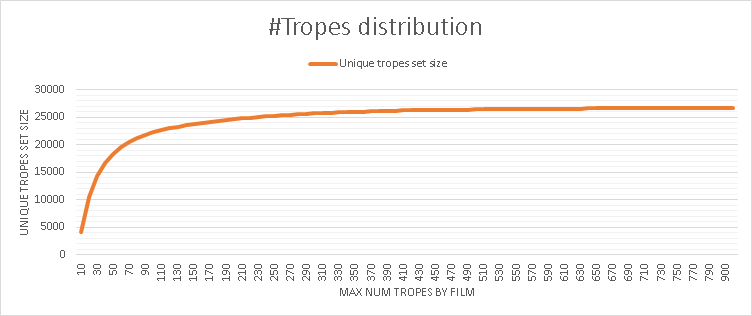
\includegraphics[width=1\linewidth]{../images/tropes_distribution.png_chart.png}
	% 	\caption{}
	% 	\label{fig:tropesdistribution}
	% \end{figure}
	
	
	
	
	
	
	
	
	
	
	% How we want to solve that problem: we think that an adaptation of word2vec should be possible
	
	
	
	% One of the most important elements in NLP (Natural Language Processing) is the context where words appear inside a text. One of the most popular algorithms to associte numerical vectors to words is word2vec \cite{mikolov2013}. This algorithm use words that are before and after a target word in order to contextualize words. But, what happend if we don't have a text to start analyzing words? What happend if we only have relationships between terms like this trope appear in this film? For this type of problem we purpouse a generalization in the use of word2vec algorithm that let to build a context for related terms. 
	
	% (Talk about A Neural Network System for Transformation of Regional Cuisine Style \cite{kazama2018} and other non-NLP word2vec use like E-commerce in Your Inbox: Product Recommendations at Scale \cite{Grbovic2015} or Meta-Prod2Vec - Product Embeddings Using Side-Information for Recommendation \cite{vasile2016}
	
	% How we do it:
	% * Methodology for creating the context of every trope
	% * Methdology for representing movies using trope vector
	% * How we evaluate the goodness of the set of movies/tropes chosen.
	
	% Our results
	% * Clustering
	% * Graph representation
	% * Movie representation
	% * Example of synthetic movie generation.
	
	% More information here about non-NLP word2vec
	% https://towardsdatascience.com/embeddings-with-word2vec-in-non-nlp-contexts-details-e879b093d34d
	% Continue here
	
	\section{State of the art}
	
	\section{Methodology}
	
	1. Download TvTropes dataset \\
	2. Select films with number of tropes less than a certain number of tropes. The idea is to create a corpus with sentences constructed by permutations of sub-sets of tropes. \\
	3. Build the corpus with permutations of tropes in each film \\
	4. Build word2vec model. After that we will have a numerical vector for each trope. \\
	5. Visualize tropes vector space in order to detect clusters and possible data organization. \\ 
	6. Create a Vector for each film as the sumatory of all tropes vectors. \\
	
	
	
	
	\section{Acknowledgments}
	
	
	\bibliographystyle{iccc}
	\bibliography{iccc}
	
	
\end{document}
